\documentclass[]{scrartcl}

\usepackage{labrep}

%opening
\title{LC filters frequency analysis}
\author{Grzegorz Potocki}
\date{14 January 2024}

\begin{document}
	
\begin{center}
	\makeatletter
	\renewcommand{\arraystretch}{2.0}% for the vertical padding

\begin{tabular}{|M{\linewidth}|}
	\hline
	
	{\LARGE Poznan University of Technology}\\
	{\LARGE Institute of Electrical Engineering and Electronics}\\
	{\LARGE Electrical and Electronics Engineering Project}\\ \hline
    \multicolumn{1}{|l|}{Title: \@title }\\ \hline
	\multicolumn{1}{|l|}{Author: \@author} \\ \hline
	\multicolumn{1}{|l|}{Date: \@date} \\
	\hline
	
\end{tabular}
\makeatother
\vspace{1.5cm}
\end{center}

\section{Introduction}

\begin{flushleft}
    Filter is a circuit which task is to pass selected frequency band and attenuate signals out of the borders of frequency band. There are different types of filters designed to achieve specific objectives, and they can be broadly categorized into several types, but two most basic are low- and high- pass filters.    
\end{flushleft}

\begin{flushleft}
    Low-pass filter has a frequency band from 0 to $\omega_0$.
\end{flushleft}

\begin{figure}[H]
	\centering
	\begin{circuitikz}
    \node[draw,minimum width=2cm,minimum height=2.4cm,anchor=south west] at (0,0){black box};
    \draw
    (1.8,2.2) node [anchor=east] {3} [short,o-] to (3,2.2);
    \draw
    (3,2.2) [rmeterwa, t=V, *-*] to (3,0.2);
    \draw
    (3,2.2) [rmeterwa, t=mA] to (5,2.2)
    to [vR=$R_z$, invert] (5,0.2)
    to [short,-o] (1.8, 0.2) node [anchor=east] {1};
\end{circuitikz}
	\caption{Type $\Pi$ low-pass filter example}
	\label{fig:circuitfig_series}
\end{figure}

\begin{flushleft}
    High-pass filter has a frequency band from $\omega_0$ to infinity.
\end{flushleft}

\begin{figure}[H]
	\centering
	\begin{circuitikz}
    \draw
    (0,2) to [C=$2C$, o-] (1,2)
    to [short] (2,2)
    to [C=$2C$, -o] (3,2)
    (0,0) to [short, o-o]  (3,0);
    \draw
    (1.5,2) to [L=$L$, *-*] (1.5,0);
\end{circuitikz}
	\caption{T-type high-pass filter example}
	\label{fig:circuitfig_series}
\end{figure}

\begin{flushleft}
    For both kinds of filters there is the attenuation coefficient which is denoted as $a$. The formula for it is:
\end{flushleft}

\begin{equation}
    a=\ln{\frac{U_1}{U_2}} \text{ [Np]}
\end{equation}

\begin{flushleft}
    The value is in [Np] which stands for neper. The attenuation of 1 neper stands for decreasing the voltage or current $e$ times. It is possible to transform the result form nepers to decibels(the units from SI metric system) by using this formulas: 
\end{flushleft}

\begin{equation}
    \frac{U_1}{U_2}=e^a \text{[-]}
\end{equation}

\begin{equation}
    a=20\log{\frac{U_1}{U_2}} \text{dB}
\end{equation}

\begin{flushleft}
    For low-pass $\Pi$ type filter the formula to calculate the attenuation coefficient $a$ is:  
\end{flushleft}

\begin{equation}
    a=\text{arccos(-A)}=\text{arccosh}(-1+\omega^2\frac{LC}{2})
\end{equation}

\begin{flushleft}
    To calculate the attenuation coefficient for high-pass T-type filters there is a formula: 
\end{flushleft}

\begin{equation}
    a=\text{arccos(-A)}=\text{arccosh}(-1+\frac{1}{2\omega^2LC})
\end{equation}

\section{The process of the exercise}

\subsection{Determination of the frequency characteristics and the attenuation coefficient a of the type $\Pi$ low-pass filter}

\subsubsection{Scheme}

\begin{figure}[H]
	\centering
	\begin{circuitikz}[american voltages, american currents, european resistors]
    \node[draw,minimum width=1.2cm,minimum height=2cm,anchor=south west] at (0,0){};
    \draw
    (-1, 1.5) [short, o-] to (0, 1.5) node [anchor=west] {G};
    \draw
    (-1, 0.5) [short, o-] to (0, 0.5);
    \draw
    (1.2, 0.6) node [anchor=east] {f} [short] to (1.4, 0.3) 
    to [short] (1.4, -0.4)
    (1.2, -0.4) to [short] (1.6, -0.4);
    \draw
    (1.2, 1.4) to (1.8, 1.4)
    to [short] (1.8, 2.4)
    to [short] (3, 2.4)
    to [C,l_=$C$] (6, 2.4)
    to [L,l_=$L$] (9, 2.4)
    to [short] (11, 2.4)
    to [rmeterwa, t=$V_R$] (11, -0.4)
    to [short] (1.8, -0.4)
    to [short] (1.8, 0.6)
    to [short] (1.2, 0.6)
    (9, 2.4) to [R=$R$,*-*] (9, -0.4)
    (3, 2.4) to [rmeterwa, t=$V_G$, *-*] (3, -0.4)
    (3.5, 2.4) to [short, *-] (3.5, 3.5)
    to [rmeterwa, t=$V_C$] (5.5, 3.5)
    to [short, -*] (5.5, 2.4)
    (6.5, 2.4) to [short, *-] (6.5, 3.5)
    to [rmeterwa, t=$V_L$] (8.5, 3.5)
    to [short, -*] (8.5, 2.4);
\end{circuitikz}
	\caption{Type $\Pi$ low-pass filter circuit}
	\label{fig:circuitfig_series}
\end{figure}

Data: $U_1$=5[V], L=90[mH], C/2=103,2[nF], R=k=660[$\Omega$], R=1000[$\Omega$] 

\subsubsection{Measurement process}

Connect the system shown in point 9.2.1.1. Measure the voltage U2 (keeping the voltage U1 at the set level: 5 V), changing the generator frequency (in the range 50 Hz - 10 kHz) so that the measuring points (voltage U2) are evenly distributed (pay special attention to the resonance occurring in the system). Perform the measurements with two load resistances and write the results in Table 9.1. For each measuring point, calculate the U1/U2 ratio and the value of the damping coefficient a. Provide the results of the calculations in Table 9.1.

\begin{table}[hptb]
	\centering
	\caption{Measurements of series circuit}
	\label{tab:tab1}
	\begin{tabular}{|c|c|c|c|c|}
		\hline
		No. & Frequency [\unit{\hertz}] & $U_R$ [\unit{\volt}] & $U_L$ [\unit{\volt}] & $U_C$ [\unit{\volt}] \\   
		\hline
		1& 10800 & 1.35 & 5.25 & 4.02\\
		\hline
		2& 10600 & 1.44 & 5.49 & 4.36\\
		\hline
		3& 10400 & 1.53 & 5.70 & 4.705\\
		\hline
		4& 10200 & 1.62 & 5.92 & 4.867\\
		\hline
        5& 10000 & 1.709 & 6.117 & 5.244\\
		\hline
        6& 9800 & 1.787 & 6.264 & 5.609\\
		\hline
        7& 9600 & 1.8465 & 6.332 & 5.915\\
		\hline
        8& 9475 & 1.87 & 6.326 & 6.077\\
		\hline
        9& 9375 & 1.88 & 6.288 & 6.175\\
		\hline
        10& 9325 & 1.882 & 6.258 & 6.21\\
		\hline
        11& 9300 & 1.881 & 6.23 & 6.22\\
		\hline
        12& 9275 & 1.8812 & 6.217 & 6.24\\
		\hline
        13& 9225 & 1.878 & 6.17 & 6.27\\
		\hline
        14& 9125 & 1.866 & 6.06 & 6.397\\
		\hline
        15& 9000 & 1.84 & 5.88 & 6.295\\
		\hline
        16& 8800 & 1.77 & 5.526 & 6.195\\
		\hline
        17& 8600 & 1.677 & 5.107 & 6.009\\
		\hline
        18& 8400 & 1.574 & 4.66 & 5.76\\
		\hline
        19& 8200 & 1.459 & 4.304 & 5.48\\
		\hline
        20& 8000 & 1.348 & 3.876 & 5.19\\
		\hline
        21& 7800 & 1.2426 & 3.48 & 4.90\\
		\hline
	\end{tabular}
\end{table}

\subsection{Determination of the frequency characteristics of the damping coefficient a of the T-type high-pass filter}

\subsubsection{Scheme}

\begin{figure}[H]
	\centering
	\begin{circuitikz}[american voltages, american currents, european resistors]
    \node[draw,minimum width=1.2cm,minimum height=2cm,anchor=south west] at (0,0){};
    \draw
    (-1, 1.5)  [short, o-] to (0, 1.5) node [anchor=west] {G};
    \draw
    (-1, 0.5) [short, o-] to (0, 0.5);
    \draw
    (1.2, 0.6) node [anchor=east] {f} [short] to (1.4, 0.3) 
    to [short] (1.4, -0.4)
    (1.2, -0.4) to [short] (1.6, -0.4);
    \draw
    (1.2, 1.4) to (1.8, 1.4)
    to [short] (1.8, 2.4)
    to [short] (3, 2.4)
    to [R,l_=$R$] (6, 2.4)
    to [short] (11, 2.4)
    to [rmeterwa, t=$V_{LC}$] (11, -0.4)
    to [short] (1.8, -0.4)
    to [short] (1.8, 0.6)
    to [short] (1.2, 0.6)
    (8, 2.4) to [short, *-*] (8, 2)
    (7,2) to [short] (9,2)
    to [L=$L$] (9,0)
    to [short] (7,0)
    to [C=$C$] (7,2)
    (8,0) to [short,*-*] (8, -0.4)
    (3, 2.4) to [rmeterwa, t=$V_G$, *-*] (3, -0.4)
    (3.5, 2.4) to [short, *-] (3.5, 3.5)
    to [rmeterwa, t=$V_R$] (5.5, 3.5)
    to [short, -*] (5.5, 2.4);
\end{circuitikz}
	\caption{T-Type high-pass filter circuit}
	\label{fig:circuitfig_parallel}
\end{figure}

Data: $U_1$=5[V], L=90[mH], 2C=103,2[mF], R=k=1320[$\Omega$], R=2000[$\Omega$]

\subsubsection{Measurement process}

Connect the system shown in point 9.2.2.1. Measure the voltage U2 (keeping the voltage U1 at the set level: 5V), changing the generator frequency (in the range 50Hz - 10 kHz) so that the measuring points (voltage U2) are evenly distributed (pay special attention to the resonance occurring in the system). Perform the measurements with two load resistances and write the results in Table 9.2. For each measuring point, calculate the U1/U2 ratio and the value of the damping coefficient a. Provide the results of the calculations in Table 9.2..

\begin{table}[hptb]
	\centering
	\caption{Measurements of parallel circuit}
	\label{tab:tab1}
	\begin{tabular}{|c|c|c|c|c|}
		\hline
		No. & f [\unit{k\hertz}] & $|U_R|$ [\unit{\volt}] & $|U_{LC}|$ [\unit{\volt}]\\   
		\hline
		1& 1.0 & 4.97 & 0.186\\
		\hline
		2& 1.5 & 4.989 & 0.2055\\
		\hline
		3& 2.0 & 4.926 & 0.43\\
		\hline
		4& 2.5 & 4.891 & 0.607\\
		\hline
        5& 3.0 & 4.833 & 0.868\\
		\hline
        6& 3.5 & 4.696 & 1.318\\
		\hline
        7& 4.0 & 4.180 & 2.203\\
		\hline
        8& 4.5 & 4.400 & 4.11\\
		\hline
        9& 5.0 & 3.095 & 3.30\\
		\hline
        10& 5.5 & 4.205 & 2.158\\
		\hline
        11& 6.0 & 4.526 & 1.586\\
		\hline
        12& 6.5 & 4.658 & 1.254\\
		\hline
        13& 7.0 & 4.722 & 1.039\\
		\hline
        14& 7.5 & 4.760 & 0.89\\
		\hline
        15& 8.0 & 4.787 & 0.78\\
		\hline
        16& 8.5 & 4.800 & 0.098\\
		\hline
        17& 9.0 & 4.810 & 0.63\\
		\hline
        18& 9.5 & 4.928 & 0.587\\
		\hline
        19& 10.0 & 4.929 & 0.540\\
		\hline
        20& 10.5 & 4.930 & 0.502\\
		\hline
        21& 11.0 & 4.937 & 0.469\\
		\hline
        22& 11.5 & 4.943 & 0.44\\
		\hline
        23& 12.0 & 4.950 & 0.415\\
		\hline
        24& 12.5 & 4.952 & 0.301\\
		\hline
        25& 13.0 & 4.950 & 0.370\\
		\hline
        26& 13.5 & 4.955 & 0.352\\
		\hline
        27& 14.0 & 4.955 & 0.335\\
		\hline
	\end{tabular}
\end{table}

\section{Conclusions and final comments}

\subsubsection{Draw the frequency characteristics of the filter attenuation coefficient for both load resistances}

\begin{figure}[H]
	\centering
	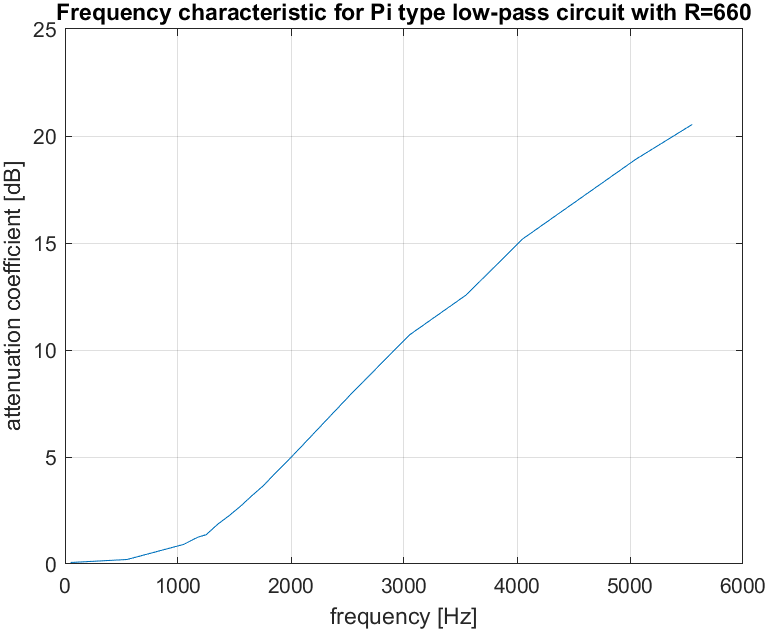
\includegraphics[width=0.7\textwidth]{Pictures/low_filter_660.png}
	\caption{Frequency characteristic graph for $\Pi$ type low-pass filter with R=660 [$\Omega$]}
	\label{fig:R=660 char}
\end{figure}

\begin{figure}[H]
	\centering
	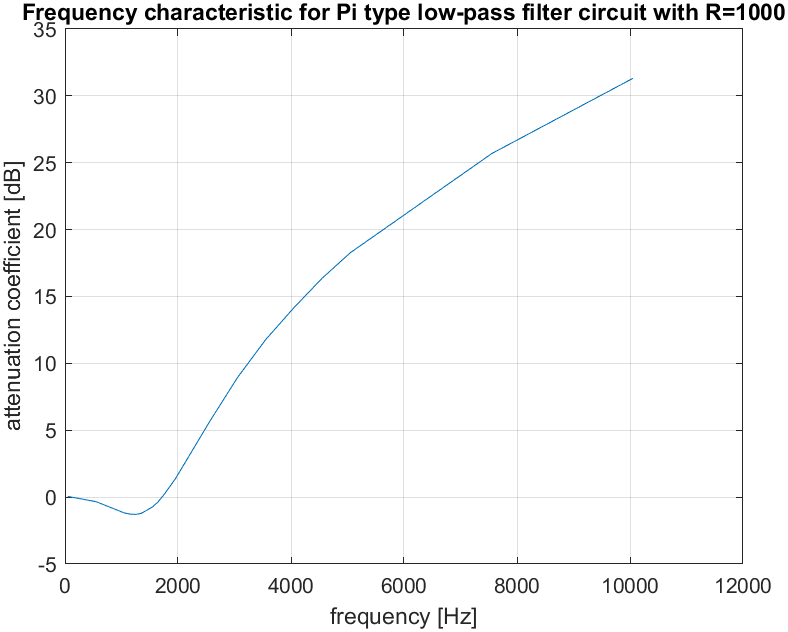
\includegraphics[width=0.7\textwidth]{Pictures/low_filter_1000.png}
	\caption{Frequency characteristic graph for $\Pi$ type low-pass filter with R=1000 [$\Omega$]}
	\label{fig:R=1000 char}
\end{figure}

\begin{figure}[H]
	\centering
	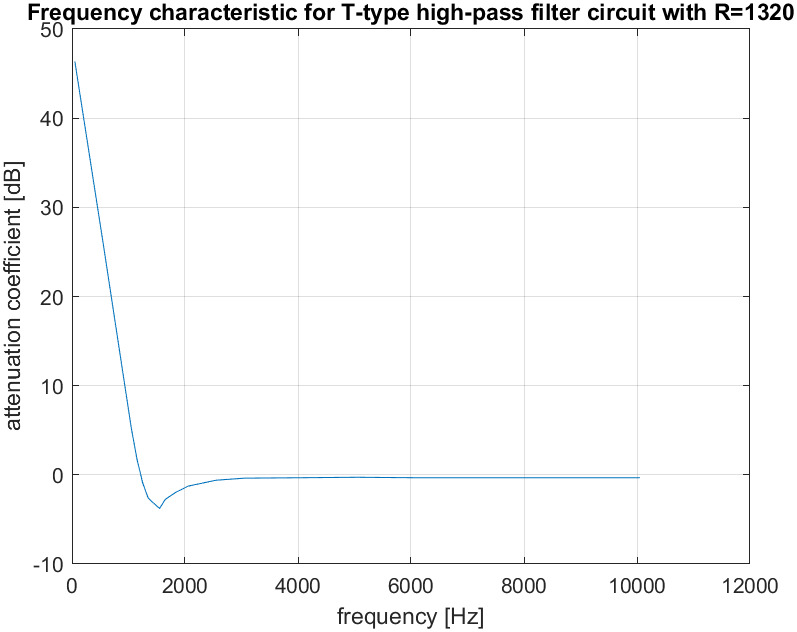
\includegraphics[width=0.7\textwidth]{Pictures/high_filter_1320.png}
	\caption{Frequency characteristic graph for T-type high-pass filter with R=1320 [$\Omega$]}
	\label{fig:R=1320 char}
\end{figure}

\begin{figure}[H]
	\centering
	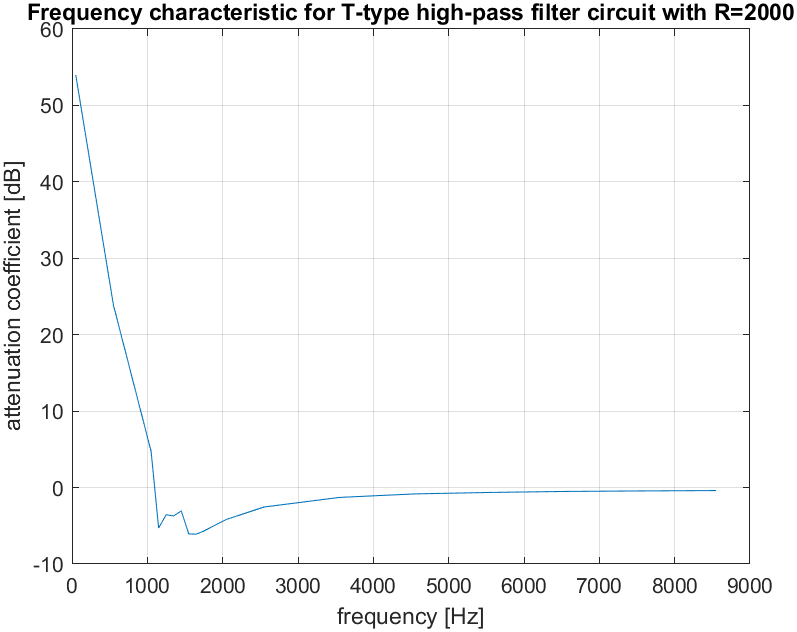
\includegraphics[width=0.7\textwidth]{Pictures/high_filter_2000.png}
	\caption{Frequency characteristic graph for T-type high-pass filter with R=2000 [$\Omega$]}
	\label{fig:R=2000 char}
\end{figure}

\subsubsection{Plot the frequency characteristics of the filter attenuation coefficient at characteristic load, obtained from theoretical calculations}

\begin{figure}[H]
	\centering
	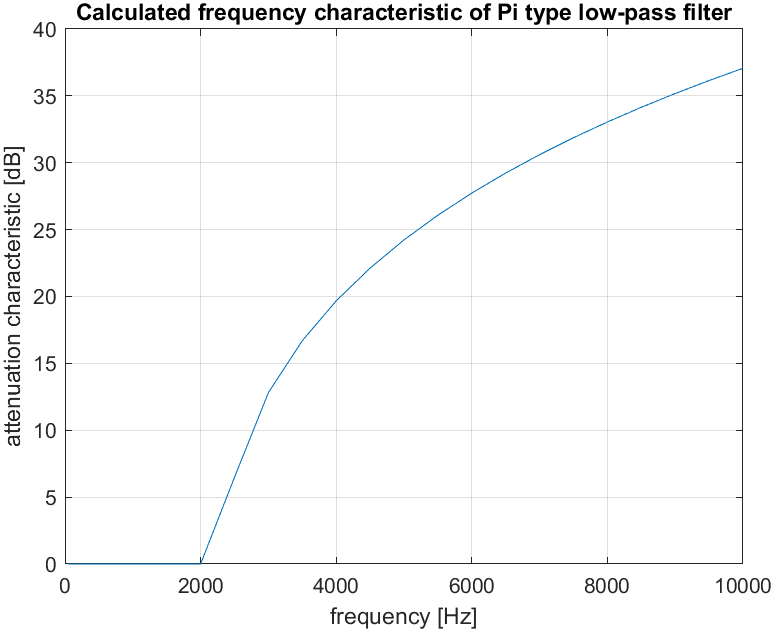
\includegraphics[width=0.7\textwidth]{Pictures/cal_low.png}
	\caption{Frequency characteristic for $\Pi$ type low-pass filter based on theoretical calculations}
	\label{fig:low-cal char}
\end{figure}


\begin{figure}[H]
	\centering
	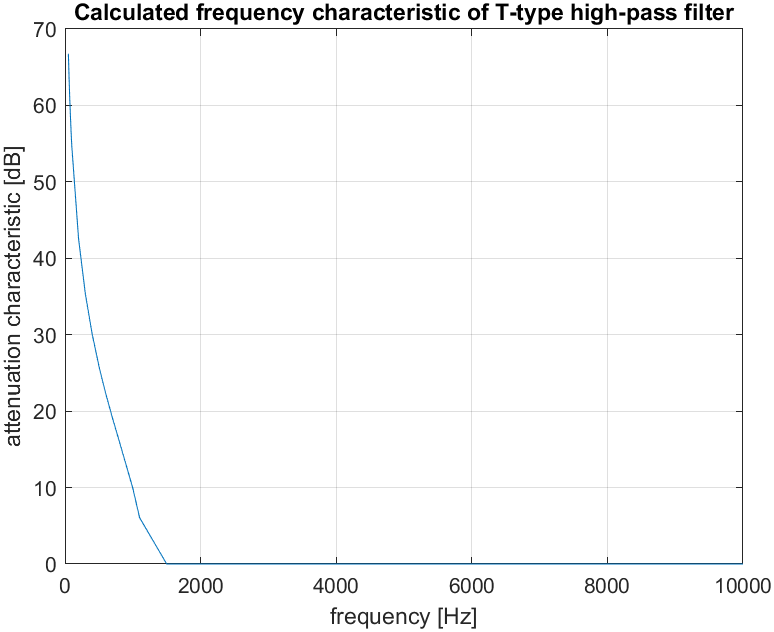
\includegraphics[width=0.7\textwidth]{Pictures/cal_high.png}
	\caption{Frequency characteristic for T-type high-pass filter based on theoretical calculations}
	\label{fig:high-cal char}
\end{figure}

\subsubsection{Compare the frequency characteristics of the damping coefficient obtained from the measurements and theoretical calculations}

\begin{figure}[H]
	\centering
	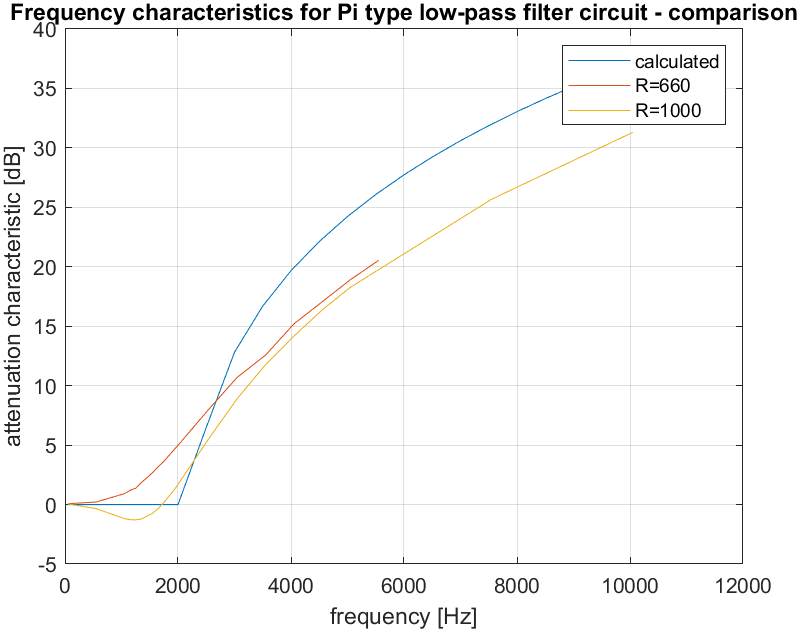
\includegraphics[width=0.7\textwidth]{Pictures/low_comp.png}
	\caption{Frequency characteristic for $\Pi$ type low-pass filter based on theoretical calculations}
	\label{fig:low-cal char-comp}
\end{figure}

\begin{figure}[H]
	\centering
	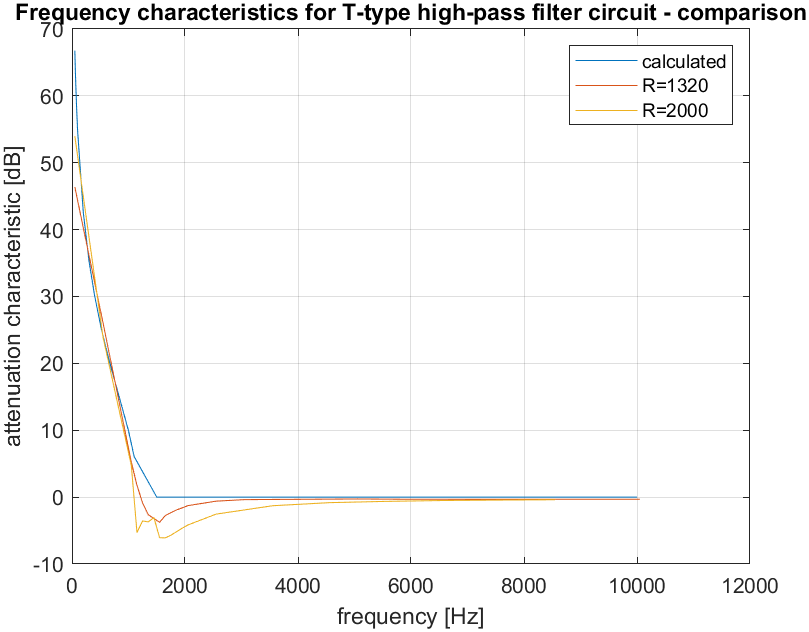
\includegraphics[width=0.7\textwidth]{Pictures/high_comp.png}
	\caption{Frequency characteristic for T-type high-pass filter based on theoretical calculations}
	\label{fig:high-cal char-comp}
\end{figure}

\subsubsection{Present conclusions and comments regarding the tested filters (performed measurements, calculation results and drawn characteristics)}

\begin{flushleft}
    In conclusion, the analysis of LC filters and their frequency response is pivotal in understanding and designing effective signal processing systems. LC filters, utilizing inductors (L) and capacitors (C), exhibit distinct characteristics in terms of their ability to pass or block specific frequencies. Moreover when the resistance was increased to 1000 $\Omega$, there were a cases when
    the $\frac{U_1}{U_2}$ ratio was less than 1. For both the T-type and $\Pi$-type filters, this had place in the band from approximately 1000 to 2000 Hz.
\end{flushleft}

\begin{flushleft}
    Therefore, when analyzing the characteristics of the attenuation coefficient a as a function of frequency f for these circuits, attention should be paid to the occurrence of negative values of the attenuation coefficient a in the mentioned frequency band. A negative value of this coefficient indicates the occurrence of amplification
    output signal (in the area of resonant frequencies).
\end{flushleft}

\end{document}